\chapter{Background}
\label{ch:background}

This chapter presents background information of the technologies and hardware used in this project. First, an introduction of RFID is provided in Section \ref{sec:rfid}. This includes a description of the technology, typical components of such systems, and potential applications in the context of this work. Then, Section \ref{sec:rssi} discusses the Received Signal Strength Indicator (RSSI) as the metric for measuring distance between readers and tags. Next, the hardware components of the project are presented in Section \ref{sec:projhard}. These are RFID readers, an active tag, and single-board computers (Raspberry Pis). Section \ref{sec:locsens} includes a discussion of location sensing techniques and evaluation criteria used throughout this project. This chapter is concluded by a survey of previous work using active RFID components to localise objects in indoor environments.

\section{Radio Frequency Identification (RFID)}
\label{sec:rfid}

Radio Frequency Identification (RFID) is a wireless technology that communicates electronically stored data between radio devices. This information is used to remotely identify objects marked with tags \cite[p. 5]{Hunt2007}. RFID uses electromagnetic waves to carry information. Such systems differ from each other by their radio frequency of operation, physical coupling method, and transmission range \cite[p. 21]{Finkenzeller2010}. Radio frequencies used in RFID range from 100kHz to 10GHz \cite{Landt2005}. The physical coupling methods in RFID classify such systems into three main categories. Close-coupling systems have a small interrogation range of up to 1cm. Remote coupled systems are capable of sensing information of up to 1m. All systems that can wirelessly read data from a marked object positioned over 1m away are called long-range systems \cite[p. 22]{Finkenzeller2010}. An RFID system has three compulsory hardware components, tags (also known as transpoders), readers (also called interrogators), and controllers.

\subsection{RFID tags}

A tag is a data-carrying device that transmits identification information in response to a received signal from a reader. RFID tags usually consist of an antenna attached to a microchip \cite[p. 2]{Want2006}. The hardware can be encapsulated in different types of enclosures. Tags come in different shapes and sizes depending on their operational environment (Figure \ref{fig:rfidtags}). RFID tags also have memory where the identification and sometimes additional information is stored. Additional data might include a delivery date of a parcel, for example. The information stored on a tag is usually only for reading. However, there are implementations of the RFID technology that benefit from writing data to a tag. For instance, a pallet might have a tag attached to it that can store the content of the pallet as it changes over time \cite[p. 8]{Hunt2007}.

\begin{figure}
	\begin{center}
		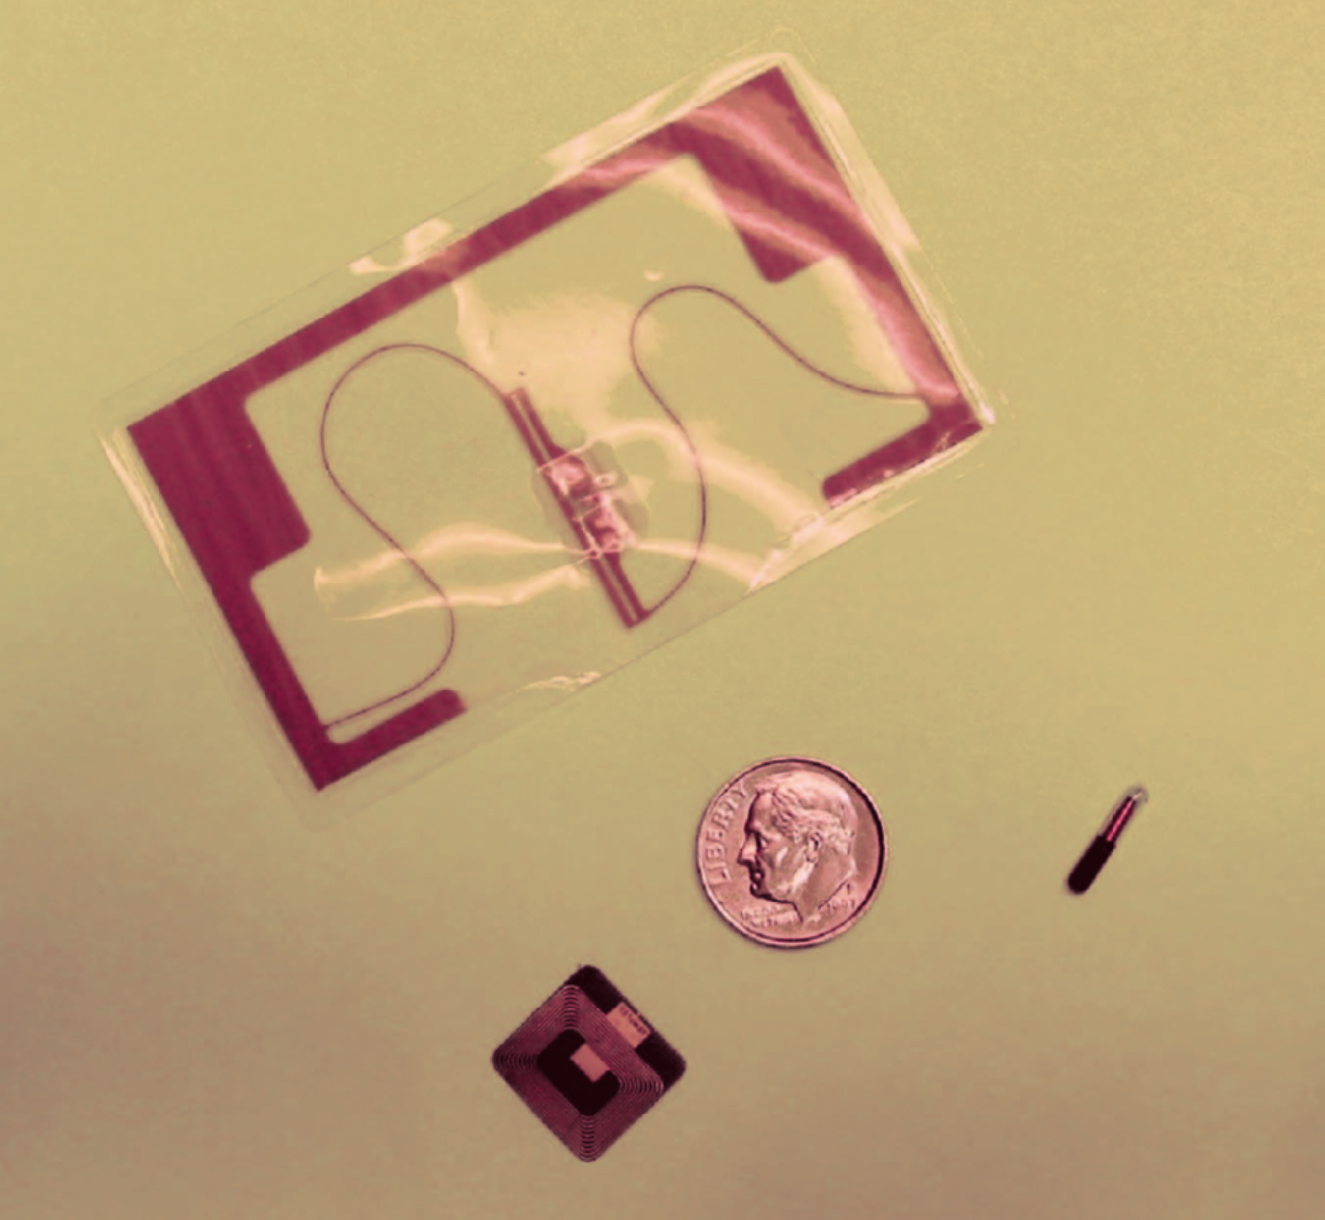
\includegraphics[width=0.5\textwidth]{figures/rfidtags}
		\caption{Three different variants of RFID tags. Figure from \cite{Want2006}.}
		\label{fig:rfidtags}
	\end{center}
\end{figure}

\subsubsection{Passive and active tags}

Tags can be classified into two main categories, passive and active. Passive tags do not require a power source. They communicate with readers by reflecting part of received radio waves, a term referred to as backscatter modulation \cite{Bolic2010}. They have a number of advantages, which include their small size, very long operational life, and low price. Nevertheless, passive tags need to be in the readers' range in order to operate. This is because passive tags obtain the power they need to supply their circuitry from an electromagnetic signal received from an RFID reader. A charge builds up into a capacitor that can power the passive tag and transmit the identification information it is storing \cite{Weinstein2005}.

In contrast, active tags require a power source in the form of a battery or are directly connected to the electrical grid \cite{Want2006}. Although their lifetime might be limited by the available energy, active tags can be read from greater distances compared to passive tags. This is because they have their own power source which enables them to emit strong signals to the readers \cite{Weinstein2005}. Compared to passive tags, active ones are larger in size and have a higher price.

\subsection{RFID readers}

A reader is a radio device that is capable of transmitting interrogation signals and capturing information send back by tags. The reader's transmission frequency specifies the operational frequency of the RFID system, which also defines their practical reading range \cite{Finkenzeller2010}. These devices usually consist of a radio frequency (RF) module that is capable of sending and receiving  signals, an antenna, and a control unit in the form of a microprocessor. RFID readers have the following main functions:

\begin{itemize}
	\item read/write data from/to an RFID tag,
	\item power a passive tag,
	\item relay the obtained information to a host computer \cite[p. 9]{Hunt2007}.
\end{itemize}

Readers are responsible for bringing additional functionality to an RFID system. This includes support for simultaneous sensing of multiple tags, authentication of tags to prevent unauthorised access to a system, and data encryption of the stored data to ensure integrity \cite[p. 10]{Hunt2007}. There is a wide range of RFID readers that differ in their operational radio frequency, range, and coupling method. These properties are formed by factors such as the specifications of the system, its budget, and security requirements \cite[p. 25]{Finkenzeller2010}.

\subsection{RFID controllers}

The third component of an RFID system is the controller or server. It is a computer that is responsible for connecting and communicating with multiple readers, aggregating any incoming data, and processing it. Readers can be connected to the server using a network or serial connection. Identification information is usually stored in a database and is used by an application software \cite[p. 11]{Hunt2007}. Figure \ref{fig:rfidsys} shows the components of a typical RFID system.

\begin{figure}[h]
	\begin{center}
		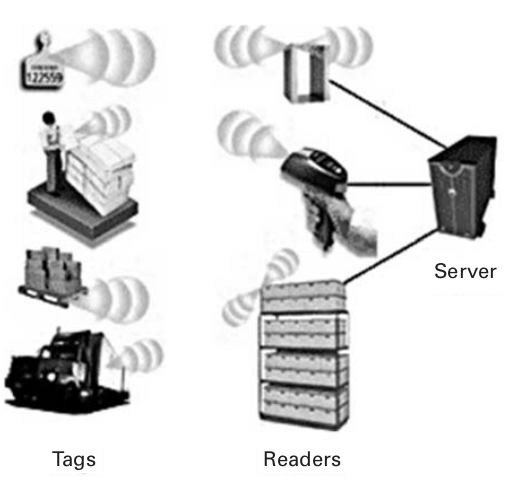
\includegraphics[width=0.5\textwidth]{figures/rfidsys}
		\caption{Components and applications of RFID. Figure from \cite[p. 20]{Rida2010}.}
		\label{fig:rfidsys}
	\end{center}
\end{figure}

\subsection{RFID applications}

RFID hardware is becoming more inexpensive, which creates a wide range of possible scenarios where this technology can be applied \cite{Nath2006}. The most widespread applications are in tracking of objects or people, in supply chain and asset management, and in health services \cite{Weinstein2005}.

Passive RFID systems can be used as an alternative and improvement of the current standard for identification of products, the barcodes.  Reading a barcode attached to an object requires a direct line of sight between a reader and a tag. In addition, barcodes can get obscured by other objects or substances, which hinders the identification process. RFID solves these disadvantages. A line of sight is not required when reading data from tags attached to objects. RFID tags also support a larger set of unique IDs compared to bar codes, can be reprogrammed, and can store additional data depending on the application requirements \cite{Weinstein2005}.

In the context of this project, which is concerned with location sensing, RFID has applications in tracking important objects or personnel and trying to pinpoint their position. For example, active RFID systems can be used in hospitals to monitor the location and life cycle of patients in an indoor environment \cite{Cangialosi2007}. Expensive hospital equipment could be tracked so that it would be at the right place and time. Another possible scenario is to track school kinds while on school grounds in order to find lost children and monitor their attendance \cite{Swartz2004}.

\section{Received Signal Strength Indicator (RSSI)}
\label{sec:rssi}

Some RFID readers provide an indication of the strength of radio signals received from tags. This metric is called Received Signal Strength Indicator (RSSI). Its value is often output along with the identity information stored in a tag. It is estimated at the reader side before amplifying the received input. RSSI is a unitless measurement of the power of the received signal represented as a positive value with certain resolution range. A resolution of three bits gives a precision of eight possible values for RSSI. This means that there are eight different steps of estimating how far a tag is. A resolution of eight bits, supported by the project hardware, lets readers output values between 0 and 255 giving a better approximation of the distance between a reader and a tag. 

\subsection{RSSI and RSS}
\label{subsec:rssiandrss}

RSSI is not to be confused with the Received Signal Strength (RSS), on which RSSI is based. RSS is usually measured in dBm\footnote{dBm - Power ratio in decibels of power referenced to one milliwatt (mW) - \url{http://en.wikipedia.org/wiki/DBm}}. It represents the attenuation of a received signal and is a function of the distance between a receiver and transmitter \cite{Bouet2008}. In WiFi, the 802.11 standard does not define the relationship between RSSI values and reported signal power levels. It is up to the manufacturers to provide a conversion function or table that specifies range and accuracy of the RSS values and how these translate into a RSSI range between zero and a maximum value \cite{Lui2011}. The above applies to RFID, which is also a radio technology. 

\subsection{RSSI and distance}
\label{subsec:rsssianddist}

A third relationship is the one between RSSI and distance. In other words, it is the problem of using RSSI reader measurements to estimate the distance separating a receiver and transmitter. More importantly, one might ask whether RSSI is a reliable parameter for localisation algorithms in wireless networks. This is not the main question that this work is concerned with. However, the reliability of this measure is of prime importance because here position estimation relies solely on this parameter. 

On the one hand, there are studies that test the reliability of both RSS and RSSI for location sensing \cite{Elnahrawy2004, Parameswaran2009}. These concluded that the limitations of determining inter nodal distances are fundamental. On the other hand, signal strength is readily available in devices today, which creates attractive opportunities for estimating position without any additional hardware. Indeed, there are a number of WiFi-based systems that rely on received signal strength including the Horus WLAN location system \cite{Youssef2005}, the EZ localisation system \cite{Chintalapudi2010}, an indoor location system using trilateration \cite{Cook2005}.

\subsection{How RSSI fits in this project}

Although RSSI is not considered a reliable measure for distance due to the physical properties of radio waves and due to cluttered and dynamic indoor environments, the aforementioned systems show that researchers and engineers try to get the best of what already is provided. In the same manner, this work uses RSSI reader measurements as a basis for location sensing. This is done using a translation table that converts RSSI into a distance metric. The methods used and the challenges faced are discussed in Section \ref{sec:rssitodist}.

\section{Project Hardware}
\label{sec:projhard}

This project combines three types of hardware. The first is active RFID devices, the second - single-board computers, and the last is a commodity network infrastructure. The main hardware components can be seen on Figures \ref{fig:projrfid} and \ref{fig:projcomp}. The following subsections present these devices and their specifications. Details on how the components are combined in forming the resulting system are given section \ref{sec:hardset}. 

\begin{figure}[h]
	\begin{subfigure}[b]{0.5\textwidth}
		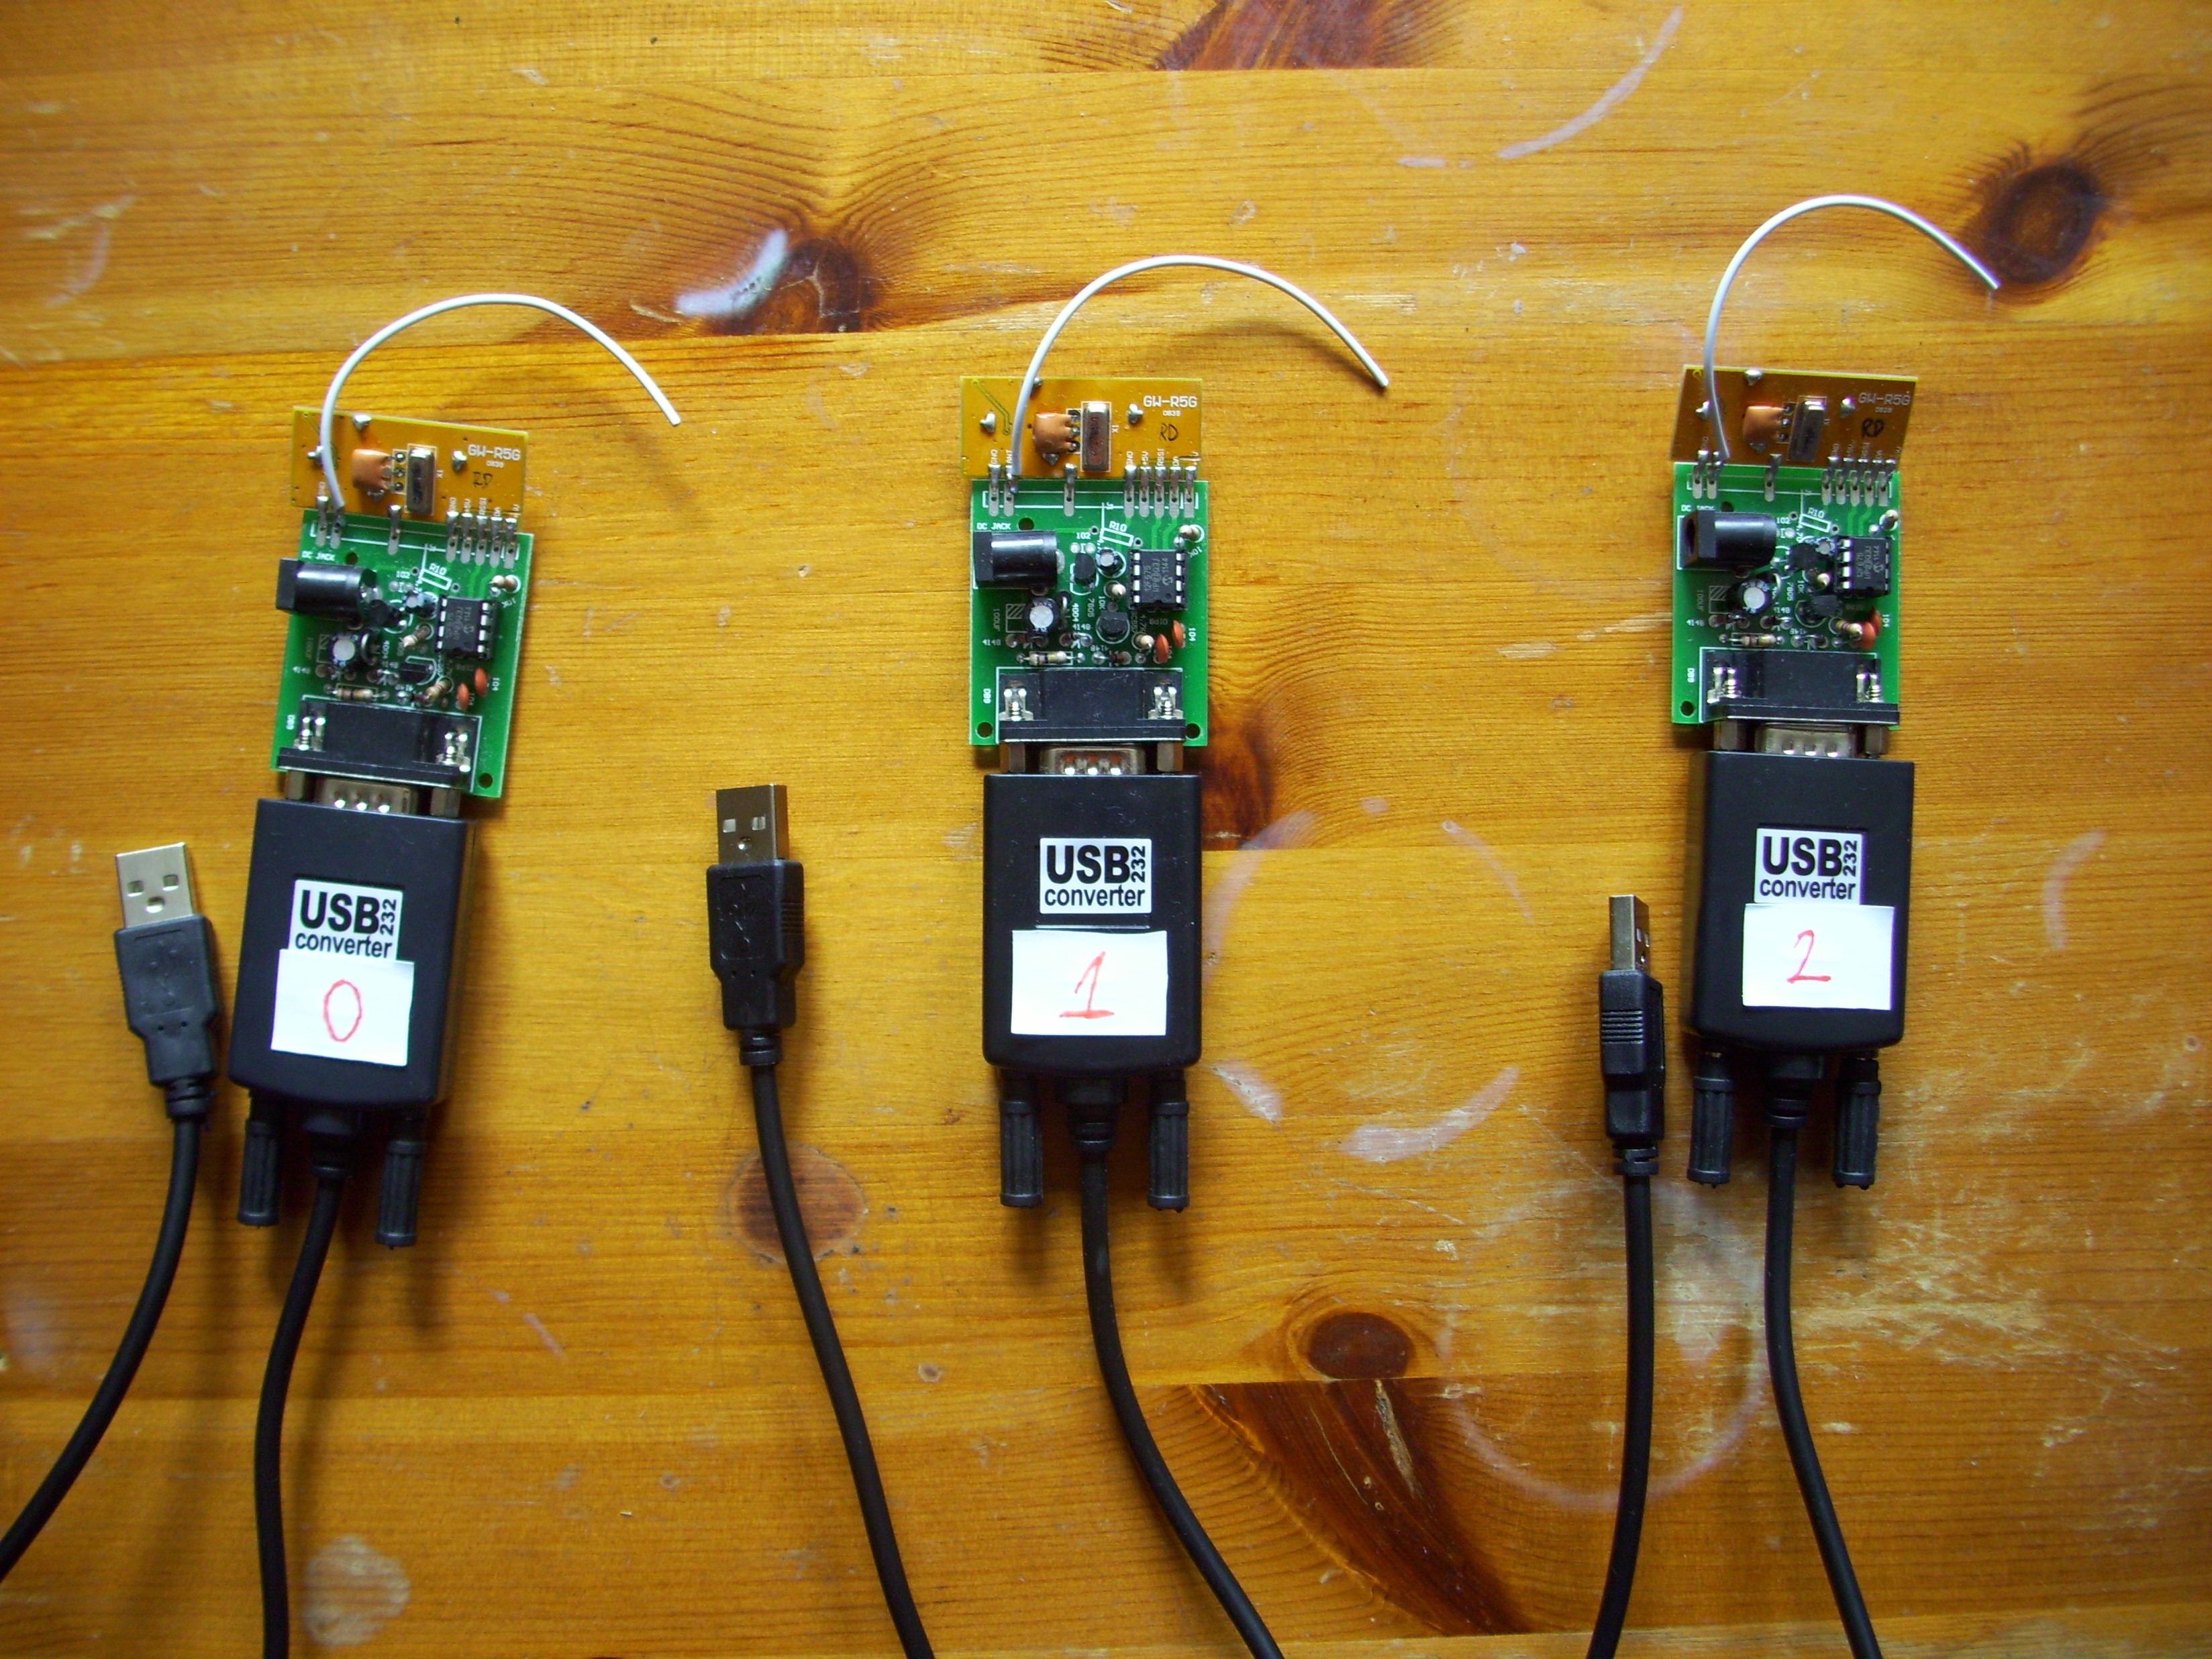
\includegraphics[width=\textwidth]{figures/readers}
		\caption{Three active RFID readers}
		\label{fig:projread}
	\end{subfigure}
	\begin{subfigure}[b]{0.5\textwidth}
		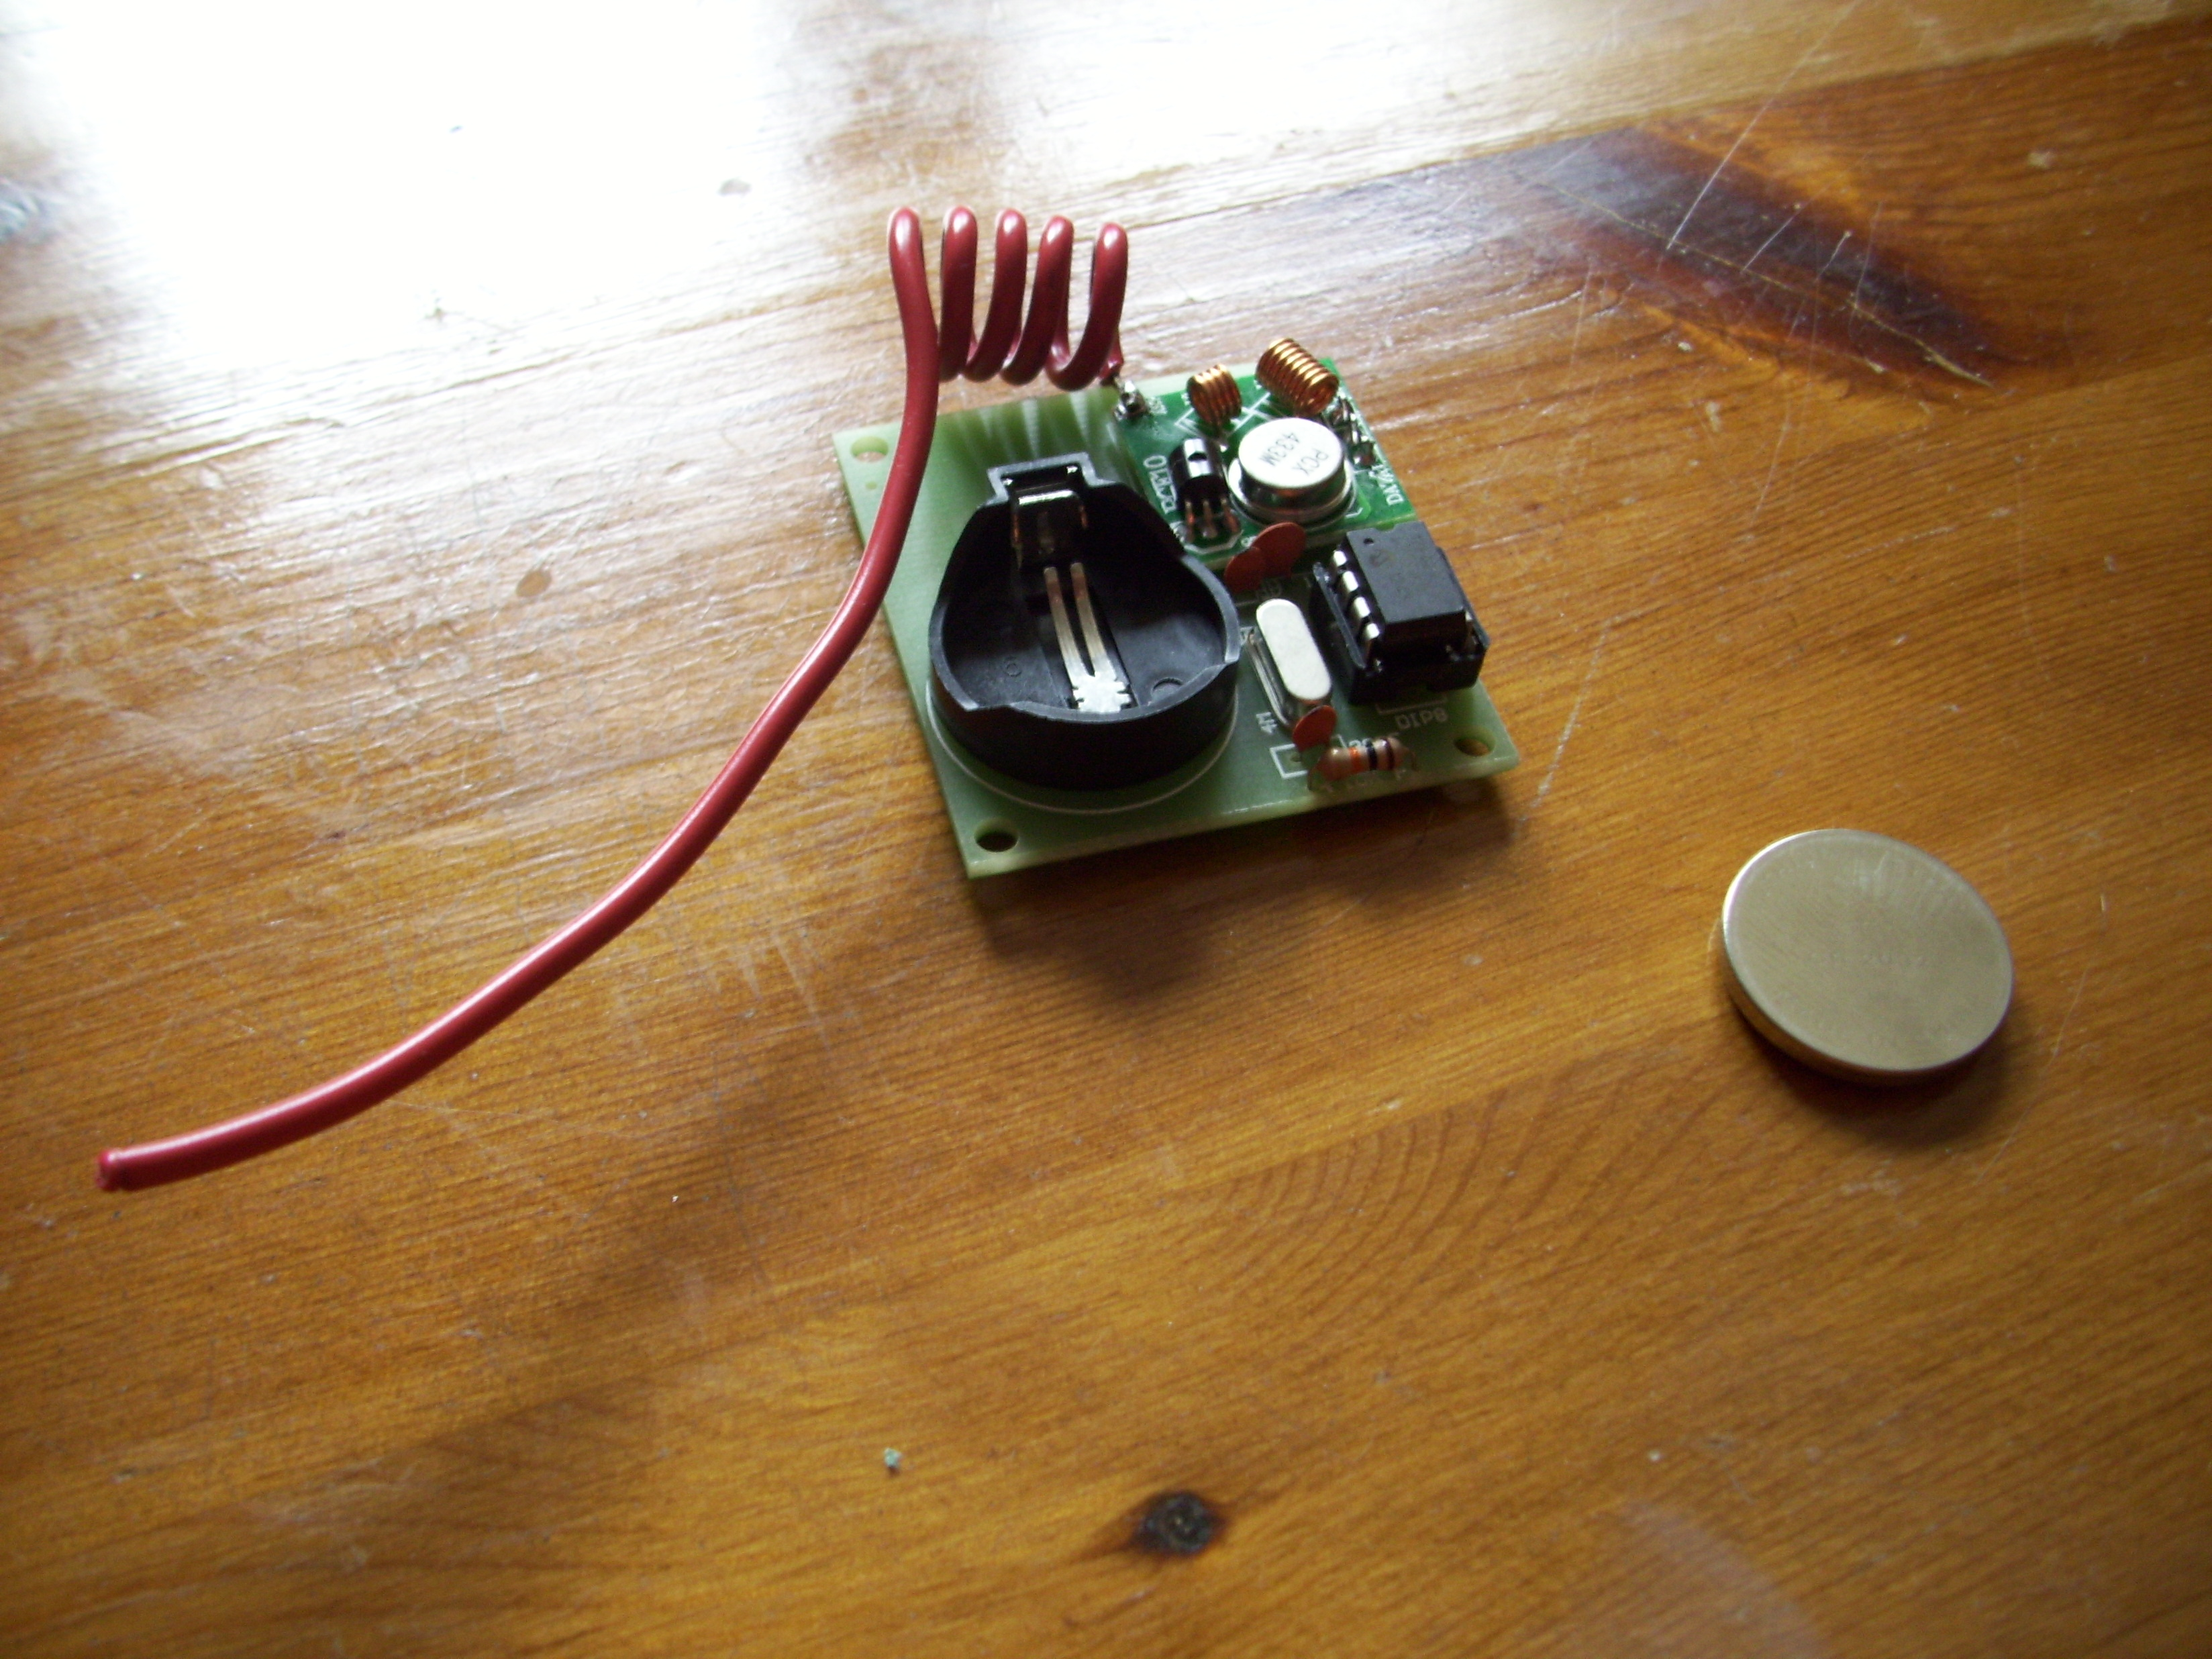
\includegraphics[width=\textwidth]{figures/tag}
		\caption{One active RFID tag}
		\label{fig:tag}
	\end{subfigure}
	\caption{RFID hardware used in this project.}
	\label{fig:projrfid}
\end{figure}


\subsection{RF9315R-u Active RFID 8 Meters Receiver with RSSI Module}
\label{subsec:receiver}

The project uses three active RFID readers containing RSSI modules. Figure \ref{fig:projread} shows the three readers, where each is connected to a serial to USB converter that offers a convenient interface to any computer with USB ports. For a discussion of the problems encountered while using the converters refer to \ref{subsec:sertousb}. 

The readers are superheterodyne receivers meaning they convert received signals to an intermediate frequency that is more convenient to process and gives a more stable design. The readers operate at 315 MHz, which lies in the lower band of Ultra High Frequency (UHF). Such waves propagate mainly by line-of-sight. They are blocked by large objects such as buildings, but can penetrate through a few building walls, which is enough for indoor location sensing. UHF are also sensitive to antenna orientations \cite[p. 15]{Hunt2007}.

The readers get their power supply from a serial or USB connection (when serial to USB converter is used). The readers have a DC 9V socket that can be used to power the devices in case the above connections are not able to supply sufficient power. The receiver devices have a built-in watchdog timer of 2.3 seconds. The watchdog timer is used to detect hardware malfunction. The readers reset the time before it elapses to confirm that they are operating correctly. These receivers can read up to 80 tags simultaneously. There is not any anti-collision protocol. The readers rely on the tags to transmit their identification data every 2.5 to 3.0 seconds.

The RFID readers employ a simple communication protocol. The serial port settings for these devices can be seen in Table \ref{tbl:comm}. Data are send in a raw character format without data encryption. The ID of a tag, consisting of four characters, is concatenated with a RSSI measurement, which could range from 0 to 255. For a discussion on the actual RSSI ranges observed during experiments refer to \textbf{REF}. Each new reading is separated by a space character. A sample input from the RFID readers is illustrated on Figure \ref{fig:comm}. 

\begin{table}[h]
	\centering
	\begin{tabular}{ | m{4cm} || m{4cm} | }
		\hline
		\textbf{Parameter}		& \textbf{Value} \\ \hline
		Baud rate				& 9600 bits per second \\ \hline
		Data bits				& 8 bits \\ \hline
		Stop bits				& 1 bit \\ \hline
		Parity					& None \\ \hline
		Flow control			& None \\ \hline
	\end{tabular}
	\caption{Serial port parameter settings to communicate with the readers.}
	\label{tbl:comm}
\end{table}

\begin{figure}[h]
	\begin{center}
		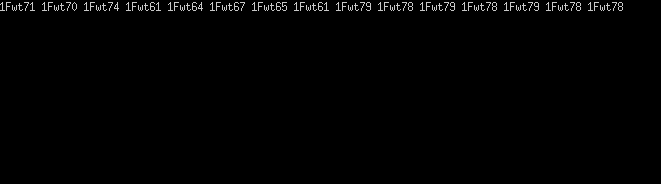
\includegraphics[width=1\textwidth]{figures/com}
		\caption{RFID reader input on a communication port. The first four characters are the ID of a tag. The number concatenated to the ID is the RSSI value. Individual readings are separated by a space character.}
		\label{fig:comm}
	\end{center}
\end{figure}

The integrated RSSI module measures the received radio frequency signal over a range of 60 dBm. The manufacturer specifies that RSSI values vary between units\footnotemark[2].  Figure \ref{fig:rssi} shows how the radio frequency signal level on the $x$ axis changes against the RSSI voltage on the $y$ axis. In can be observed that the signal levels can be effectively measured between -55 and -115 dBm giving a range of 60 dBm. The readers' specifications described above are summarised in Table \ref{tbl:reader}. These reader devices are a good fit for this project because of their low price, RSSI modules with good resolution, active RFID type, and USB connectivity.

\begin{figure}[h]
	\begin{center}
		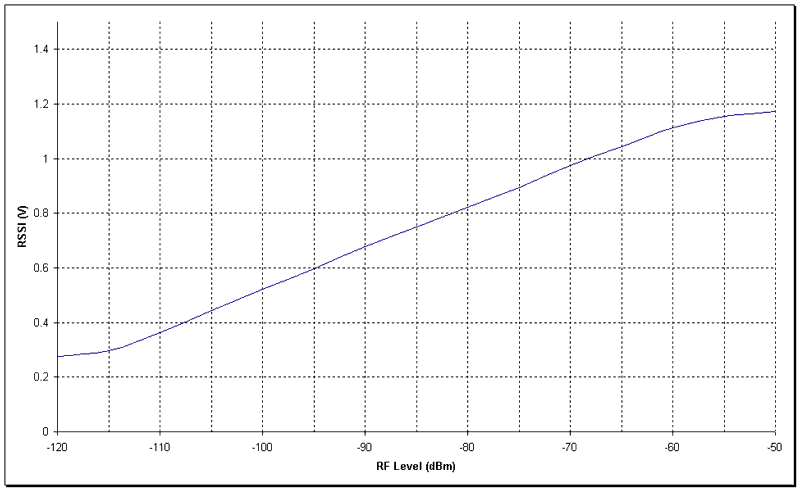
\includegraphics[width=0.7\textwidth]{figures/rssi}
		\caption{A plot of radio frequency signal levels against RSSI voltage. Figure from product website\protect\footnotemark[2].}
		\label{fig:rssi}
	\end{center}
\end{figure}

\begin{table}[h]
	\centering
	\begin{tabular}{ | m{4cm} || m{7cm} | }
		\hline
		\textbf{Specification}	& \textbf{Value} \\ \hline
		Dimensions				& 4cm x 6cm x 1.8cm \\ \hline
		Operating Temperature	& 0 - 50$^\circ$ C	\\ \hline
		Operating Frequency		& 315 MHz	\\ \hline
		Incoming signal range	& 60 dBm \\ \hline
		Power source			& Serial / USB port, DC 9V socket \\ \hline
		Communication			& RS-232 serial port \\ \hline
		Watchdog timer			& 2.3 seconds \\ \hline
		Simultaneous reads		& 80 tags	\\ \hline
		Reader control			& No control protocol \\ \hline
		Data representation		& Raw character data, No data encryption	\\ \hline
		Data output				& ID: 4 characters + RSSI: 0-255 \\ \hline
		Price					& US \textdollar 49.95 \\ \hline
	\end{tabular}
	\caption{Specifications of RF9315R-u active RFID reader. Table from product website\protect\footnotemark.}
	\label{tbl:reader}
\end{table}
\footnotetext{Ananiah Electronics active RFID reader - \url{http://www.ananiahelectronics.com/RF9315R-u.htm}.}


\subsection{RF8315T Active RFID 8 Meters Transmitting Module}

The active tag is a radio transmitting device that sends out its unique four character identification every 2.5 $\pm$ 0.5 seconds. Figure \ref{fig:tag} shows the active RFID tag used in this work. Its transmission time is around 11ms giving a small probability of tags' signals colliding. The tag can use CR2025 and CR2032 batteries as a power supply. It can operate between 5,000 and 7,000 hours with a single battery. The tag consumes most of its power (4mA) while transmitting. During the rest of the time, the tag stays into hibernation mode using only 18uA.

The effective transmission range of the tag is estimated at eight meters by the manufacturer. For range measurements conducted during this project refer to \textbf{REF}. The tag arrived without an antenna. According to the specifications, to achieve its effective range, the antenna should have a 8mm coil diameter and 2cm coil length. The construction of the antenna is discussed in section \ref{subsec:antdes}. The tag specifications described above are summarised in Table \ref{tbl:tag}. This RFID tag was chosen for this project because of its low price, transmission range, portable size, low power consumption, and matching operating frequency to the readers.

\begin{table}[h]
	\centering
	\begin{tabular}{ | m{4cm} || m{7cm} | }
		\hline
		\textbf{Specification}	& \textbf{Value} \\ \hline
		Dimensions				& 4cm x 5cm x 1.8cm \\ \hline
		Operating Temperature	& 0 - 50$^\circ$ C	\\ \hline
		Operating Frequency		& 315 MHz	\\ \hline
		Power source			& CR2025 / CR2032 battery \\ \hline
		Battery life			& 5,000 / 7,000 hours \\ \hline
		Power consumption		& 4mA when transmitting, 19uA when idle \\ \hline
		RF output power			& $<$ 2mW \\ \hline
		Effective range			& 8 meters with 8mm coil diameter, 2cm long antenna \\ \hline
		Data output				& ID: 4 characters \\ \hline
		Price					& US \textdollar 19.95 \\ \hline
	\end{tabular}
	\caption{Specifications of RF8315T active RFID tag. Table from product website\protect\footnotemark.}
	\label{tbl:tag}
\end{table}
\footnotetext{Ananiah Electronics active RFID tag - \url{http://www.ananiahelectronics.com/RF8315T.htm}.}


\subsection{The Raspberry Pi}

A single-board computer is a computer that is built on a single circuit board. It features most of the components of a personal computer. It has a processor, memory, storage, different microprocessors, and input/output interfaces. The Raspberry Pi is a particular implementation of a single-board computer. This project uses three such devices in order to construct a location sensing system. Figure \ref{fig:pis} shows these computers.

The Raspberry Pi has compact dimensions and is low on weight. It consumes little power, but has enough processing power, memory, and storage to run a standard operating system, such as the Raspbian Linux. The Raspberry Pi has two USB 2.0 ports as well as an Ethernet network port. In addition, the Pi has some characteristics of a development board employing a General Purpose Input/Output (GPIO) interface, which is could be used for connecting low-level peripherals such as RFID readers. The characteristics of the Raspberry Pi make it a great candidate for this project. Its specifications are summarised in Table \ref{tbl:pi}.

\begin{table}[h]
	\centering
	\begin{tabular}{ | m{4cm} || m{6cm} | }
		\hline
		\textbf{Specification}	& \textbf{Value} \\ \hline
		Dimensions				& 86mm x 54mm \\ \hline
		Weight					& 45g \\ \hline
		Power source			& 5V MircroUSB or GPIO \\ \hline
		Power rating			& 700mA (3.5W) \\ \hline
		System on a chip		& Broadcom BCM2835 \\ \hline
		CPU						& 700MHz ARM1176JZF-S \\ \hline
		GPU						& Broadcom VideoCore IV 250MHz \\ \hline
		Memory					& 512MB \\ \hline
		Storage:				& SD card slot \\ \hline
		USB	2.0 ports			& 2 \\ \hline
		Networking				& 10/100 Ethernet \\ \hline
		Low-level peripherals	& 8 x GPIO, UART, I$^{2}$C bus, SPI bus \\ \hline
		Operating system		& Raspbian Linux \\ \hline
		Price					& US \textdollar 35 \\ \hline
	\end{tabular}
	\caption{Specifications of the Raspberry Pi Model B revision 2 single-board computer. Table from product website\protect\footnotemark.}
	\label{tbl:pi}
\end{table}
\footnotetext{The Raspberry Pi website - \url{http://www.raspberrypi.org/faqs}.}

\begin{figure}[h]
	\begin{subfigure}[b]{0.5\textwidth}
		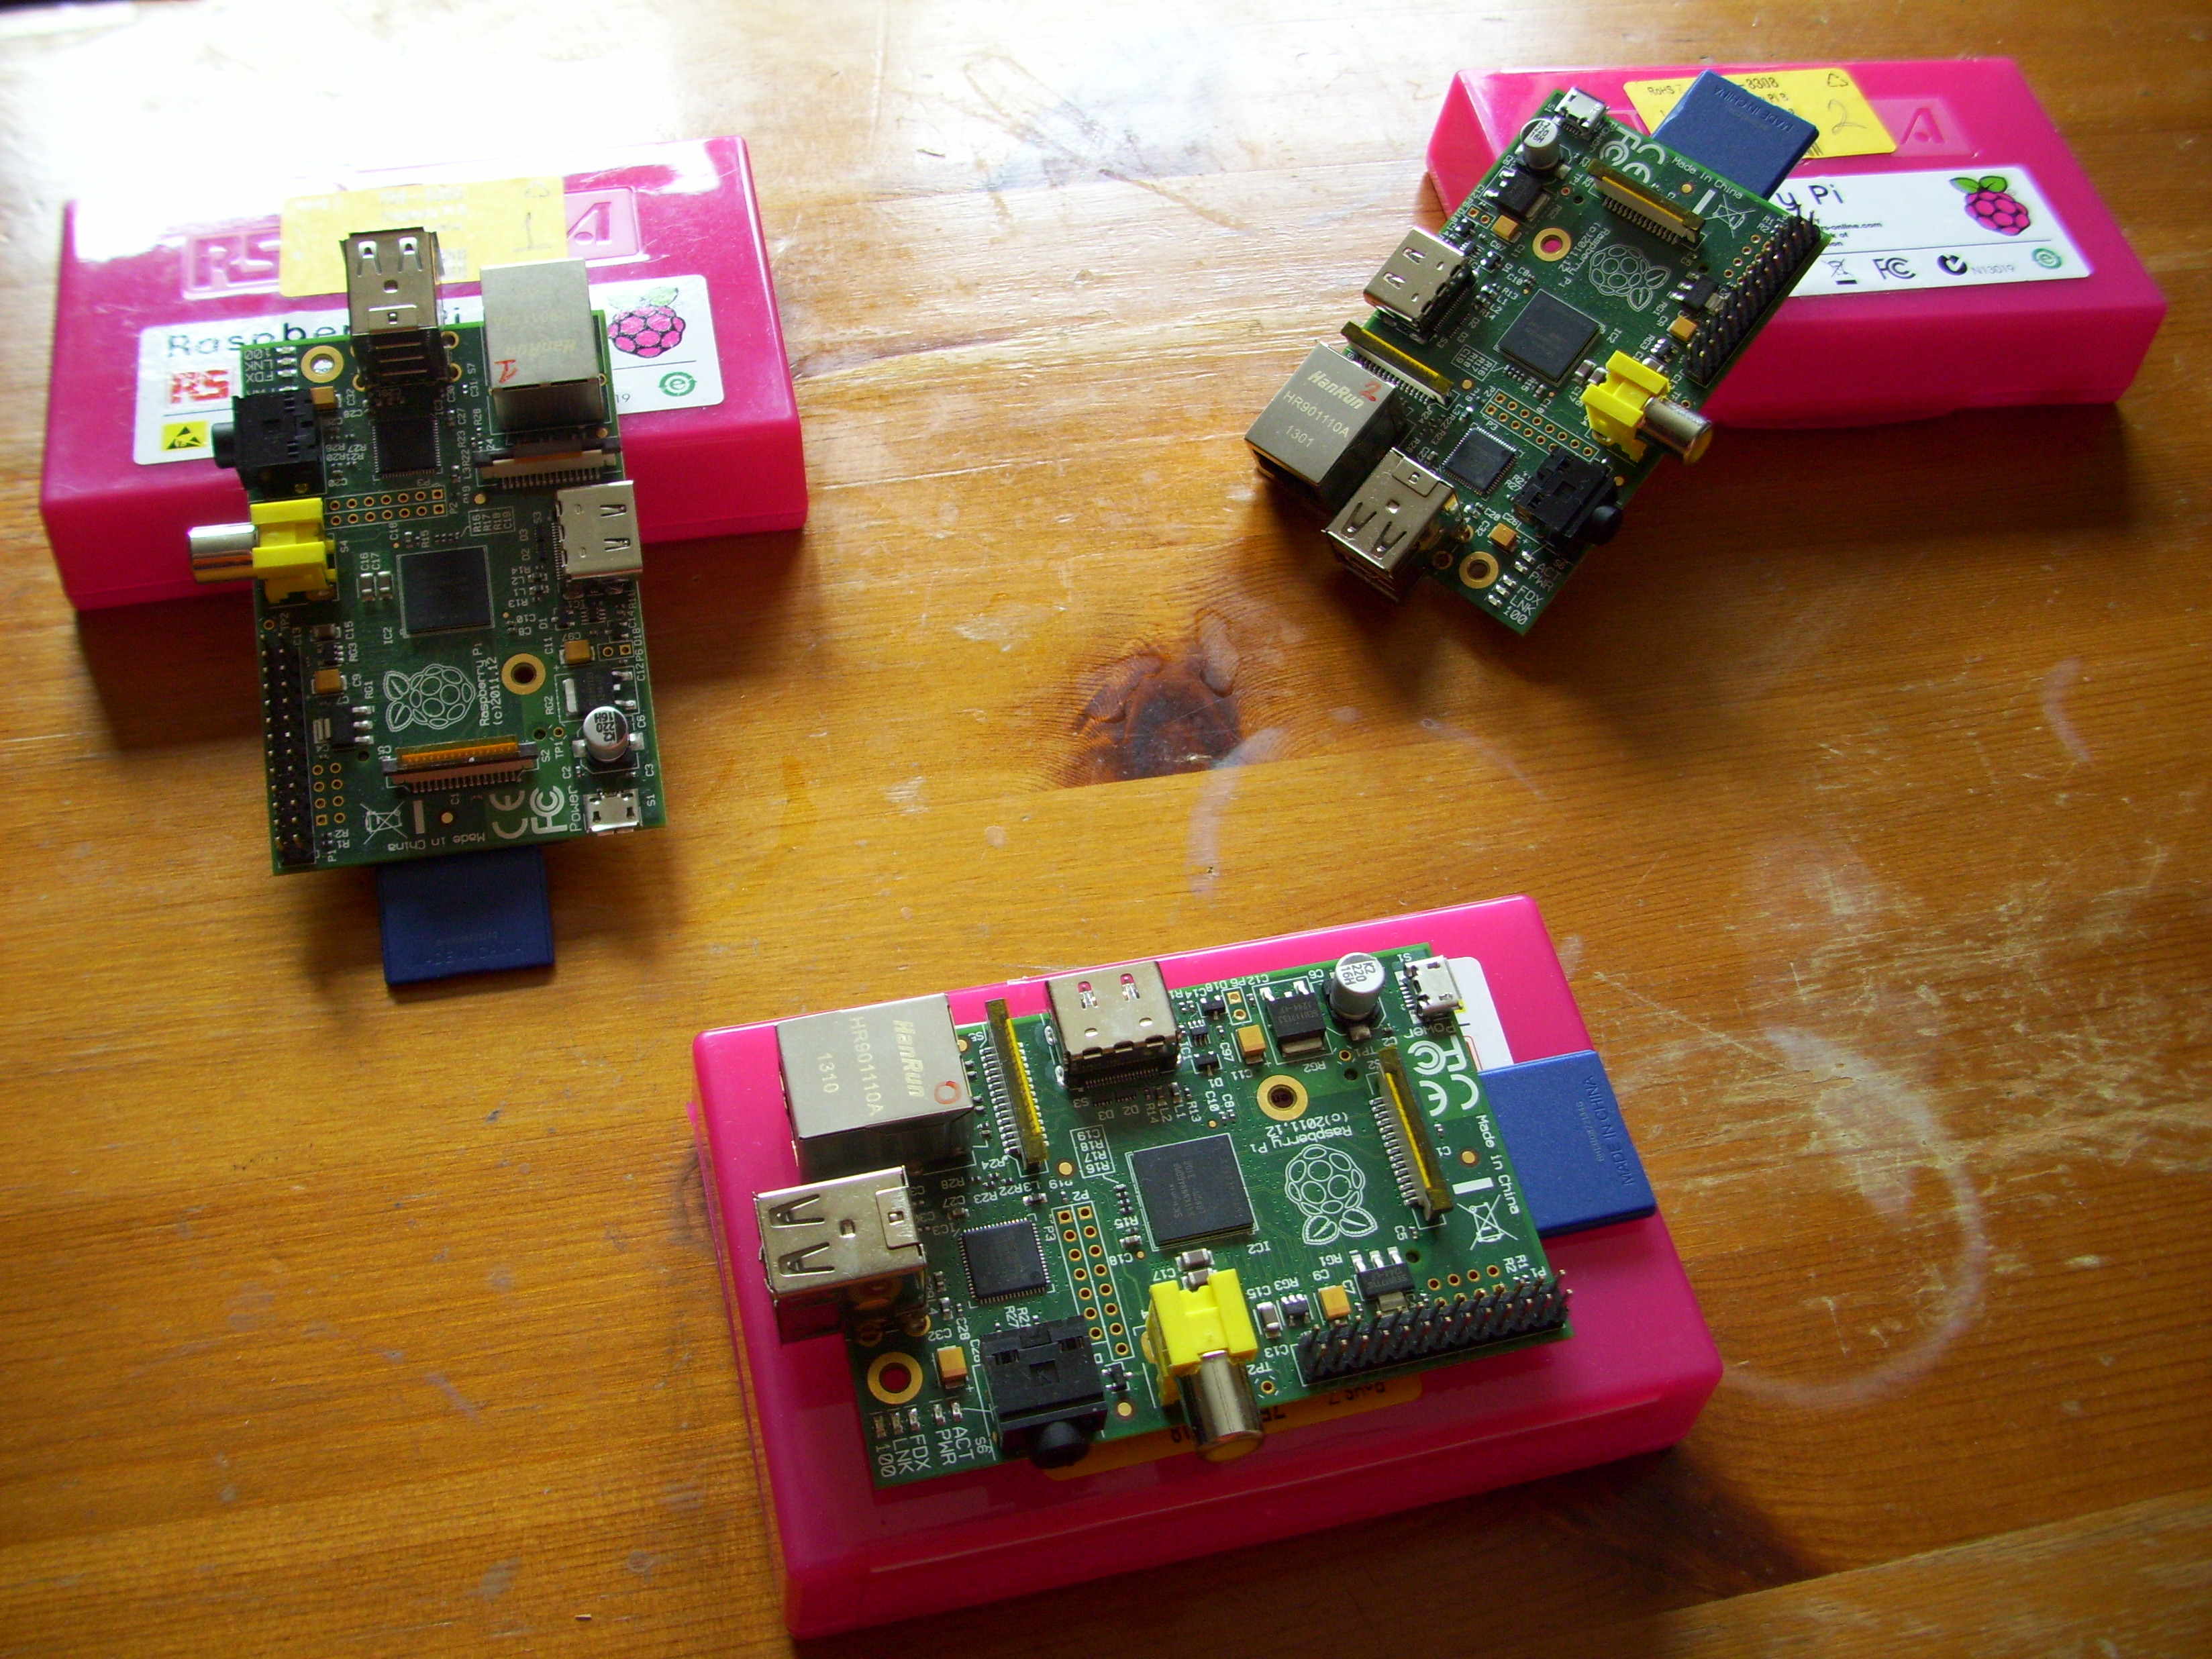
\includegraphics[width=\textwidth]{figures/pis}
		\caption{Three Raspberry Pis}
		\label{fig:pis}
	\end{subfigure}
	\begin{subfigure}[b]{0.5\textwidth}
		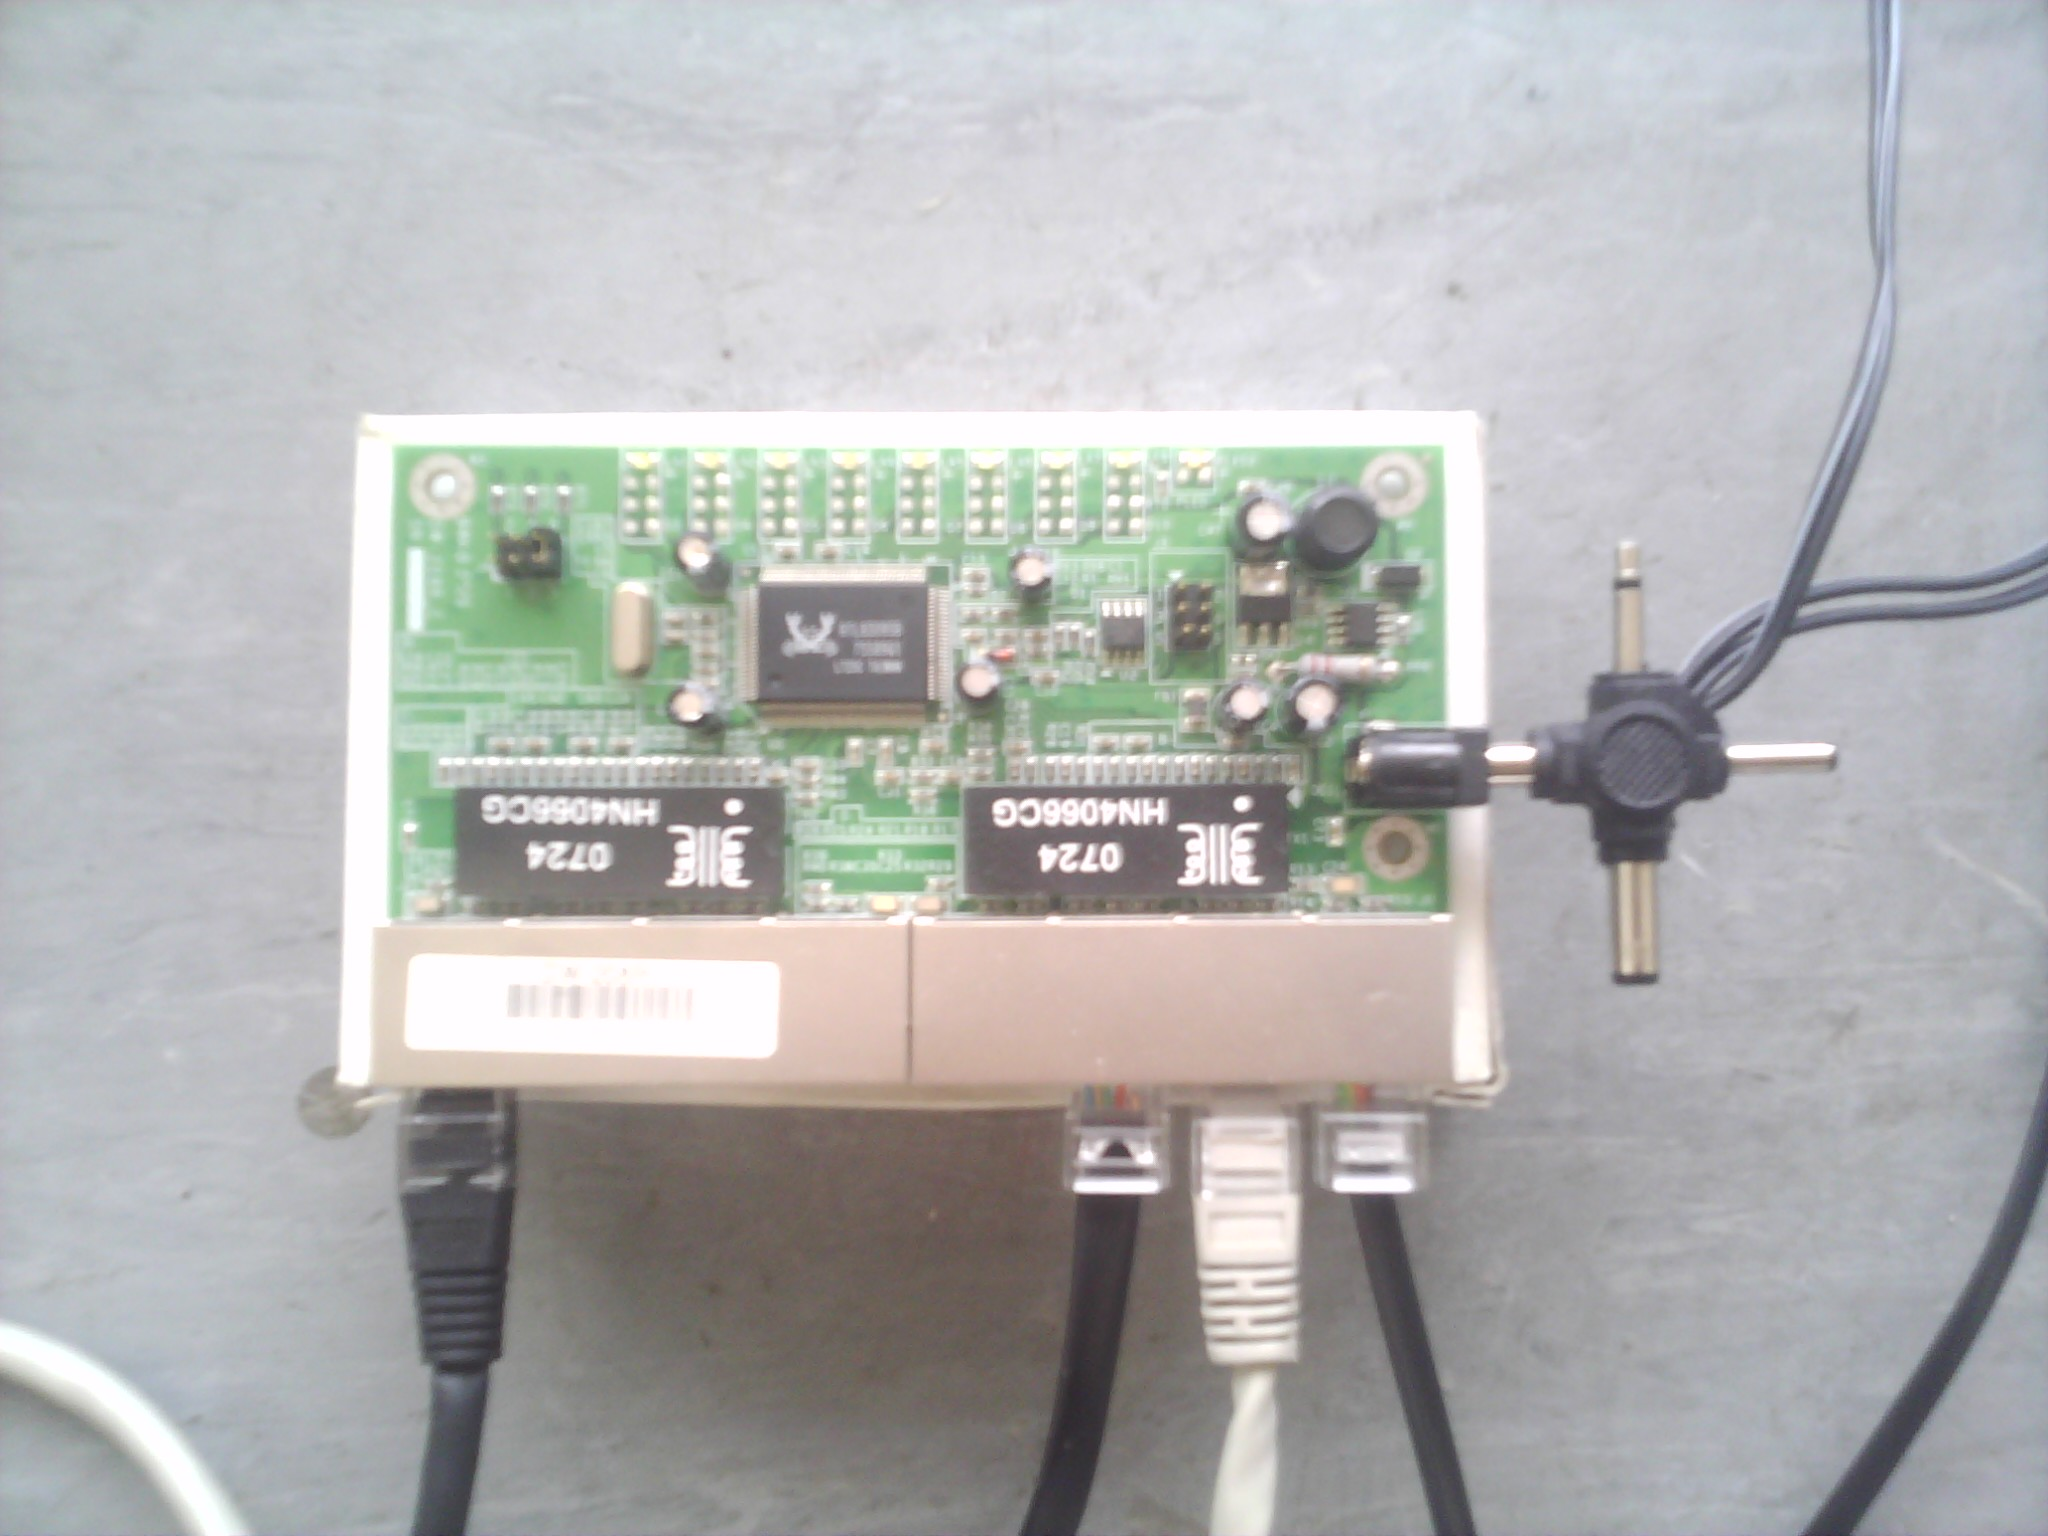
\includegraphics[width=\textwidth]{figures/switch}
		\caption{LAN switch}
	\end{subfigure}
	\caption{Computer and network hardware used in this project.}
	\label{fig:projcomp}
\end{figure}

\section{Location sensing}
\label{sec:locsens}

Estimating the position of an RFID transmitter using three receivers is the main goal of this project. This section describes a localisation technique that is suitable for the available hardware. It also defines criteria for evaluating estimated positions. 

\subsection{Trilateration}
\label{sec:trilatback}

Trilateration is a localisation technique that uses the geometric properties of triangles in order to compute locations \cite{Hightower2001c}. This technique has practical applications in surveying and global positioning systems. Trilateration requires the known locations of two or more reference nodes as well as the distance measurements between a reference node and the unknown object \cite[p. 280]{Zhang2009}. In this project, the distance from a reader to a tag is the radius of a circle that could be drawn around the reader. The intersection of circles of three readers can be used to determine the approximate location of a tag relative to the readers. In order to compute the position of an unknown object in two dimensions, trilateration requires three reference points that are non-collinear \cite{Zhang2009}. In a three dimensions case, four non-coplanar nodes and their distance measurements are needed \cite{Hightower2001c}. Figure \ref{fig:trilat} shows  a graphical representation of the concept of trilateration. Section \ref{sec:trilatmeth} presents the mathematical method for estimating the position of unknown object in three dimensions. 

\begin{figure}[h]
	\begin{center}
		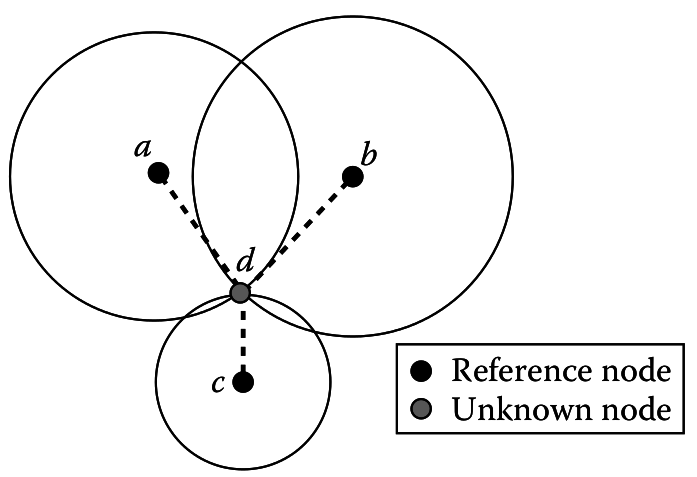
\includegraphics[width=0.55\textwidth]{figures/trilat}
		\caption{The trilateration technique for positioning an unknown node based on distance measurements from three reference nodes. Figure from \cite[p. 281]{Zhang2009}.}
		\label{fig:trilat}
	\end{center}
\end{figure}


\subsection{Evaluating an estimated position}

An important requirement for every location system is to estimate positions consistently and accurately. Hightower \cite{Hightower2001c} proposed criteria for the classification of such systems based on properties including accuracy, precision, and distribution of erroneous positions to the true one. Such metrics can be used when evaluating a location system's performance in terms of how often it locates an object within some distance of its true location. For instance, if a GPS receiver can locate its position within five meters for 90 percent of the time, then its accuracy is five meters and has a precision of 90 percent for that accuracy \cite{Hightower2001}. There is a trade-off between accuracy and precision. To achieve a higher precision, one might have to sacrifice accuracy. As a result, in order to arrive at a concise quantitative summary of these attributes, Hightower proposed to assess the error distribution accumulated during a system's operation \cite{Hightower2001}. In addition, this should be combined with other parameters such as the number of nodes in the system, the density of the infrastructure, and the size of the indoor space. In this work, these metrics are used to evaluate the localisation performance of the resulting system.

\section{Previous work}
\label{sec:prevwork}

The RFID technology is of substantial interest to researchers. Location sensing using active RFID devices is a specific subcategory of this field. Nevertheless, there have been a number of important research efforts to construct localisation systems using the available RFID hardware at that time. This section presents some of the previous work that directly relates to this project.


\subsection{SpotON}

SpotON is a fine-grained tagging technology for 3D location sensing using radio signal strength analysis \cite{Hightower2000}. The author's motivation was to develop a low cost system compared to commercial solutions available at their time. SpotON's operation involves a number of readers collecting signal strength information from active tags to determine their positions in the 3D space. It was the author's believe that the accuracy and efficiency of location sensing could be enhanced by sensor fusion, i.e. adding more sensors (accelerometers) and building proximity maps \cite{Hightower2000}.

\subsubsection{Operation}

The SpotON algorithm consists of two main parts. First, RSS measurements are converted into a distance estimation. This is done using a translation function relying on numerical variables that were identified based on observation. This function is hardware-specific and cannot be applied in this project. Second, distance measurements are used as an input to a localisation algorithm that tries to minimise RSS errors \cite{Hightower2000}. It is based on the lateration geometrical process to estimate a position for an active RFID tag.

\subsubsection{Limitations}

At the time or their research, Hightower and his colleagues were using RFID hardware with 2-bit accuracy when measuring received signal strength \cite{Hightower2000}. They identified that this accuracy is not enough to achieve the precision required for localisation in small indoor environments. The authors mentioned that 8-bit accuracy (supported by this project's hardware) could be used in the future for improved performance \cite{Hightower2000}. Another limitation was the frequency of collecting measurements. This would take between 10 and 20 seconds, which is generally too slow for monitoring real-time position changes of objects. These drawbacks were solved by creating custom RFID hardware.

\subsubsection{Results}

When localising a tagged object, the SpotON system achieved accuracy of three meters using off-the-self hardware \cite{Hightower2000}. Relying on their custom RFID devices, SpotON reported under one meter location sensing accuracy.


\subsection{LANDMARC}

LANDMARC is a 2D location sensing system that uses RFID for locating objects inside buildings. The major advantage is that it improves the overall accuracy of locating objects by using reference tags \cite{Ni2004}. The authors believed that the choice of technology and techniques is of crucial importance for the granularity and accuracy of the location information. They identified that the range of an RFID system is determined by the power available at the tags, indoor topology, and environmental conditions. Ni and his colleagues found out that instead of using a lot of readers, they can arrange a number of tags in a 2D rectangular grid to use as reference tags \cite{Ni2004}. The advantage is that tags are cheaper than readers. Also, reference tags are subject to the same environmental factors as the tags being tracked. The authors argue that the placement of readers and reference tags is very important for the accuracy of the system \cite{Ni2004}.

\subsubsection{Operation}

The core idea of LANDMARC is to select the k nearest reference tags that are closest to the unknown tag using differences in RSS measurements. Having identified the k nearest reference tags, their known positions are used to localise the unknown tag. Distances between tags are computed using Euclidean distance. The system also applies a weighing factor when computing coordinates, where small distances receive a bigger weight.

\subsubsection{Limitations}

The hardware problems of the current RFID technology were identified \cite{Ni2004}. RFID hardware used in LANDMARC did not supply signal strength directly, which resulted in unnecessary processing and sacrificed accuracy. LANDMARC took a substantial time to estimate locations. Two factors were contributing to these problems. One being the scanning time of the readers in order to collect signal strengths. The second, the time interval of a tag emitting its identification information, which could not be controlled. Ni and his colleagues also measured different power levels from two tags placed at identical positions. This resulted in unstable system behaviour.

\subsubsection{Results}

The authors experimented with different number and placement of readers, reference and tracking tags. The best setup was consisting of four readers and one reference tag per square meter resulting in an average distance error of one meter \cite{Ni2004}.

\subsubsection{Extension systems}

VIRE extends the methods used in LANDMARC by defining virtual reference tags and a proximity map that every reader records \cite{Zhao2007}. This proximity map consists of a 2D grid of reference tags where the centre of a cell is a tag. The difference in the RSS measurements between reference and unknown tag helps label cells in the proximity map so that it can be constructed. The union of individual proximity maps gives a global proximity map for the unknown tag. Experimental results showed an improvement of LANDMARC's precision between 17 and 73 percent for different scenarios and indoor environments \cite{Zhao2007}.

LANDMARC is a location sensing system that reports a two dimensional tag positions. The extended 3-D LANDMARC algorithm is a system that could localise tags in three dimensions \cite{Khan2009}. A major difference is the use of passive tags instead of active ones. This system solves some of the original limitations of LANDMARC by using hardware providing received signal strength directly. The authors rely on similar methodology, but extend computations to three dimensions. The accuracy of the system was estimated at around 0.5 meters when employing three readers, two tracking tags, and 11 reference tags in an 11 cubic meter space \cite{Khan2009}.


\section{Summary}

This chapter presented background information of the technologies and hardware used in this project. First, an introduction of RFID is provided in Section \ref{sec:rfid}.  Then, Section \ref{sec:rssi} discusses the Received Signal Strength Indicator (RSSI). Next, the hardware components of the project are described in Section \ref{sec:projhard}. Section \ref{sec:locsens} includes a discussion of location sensing techniques and evaluation criteria. This chapter is concluded by a survey of previous work relating to this project.
